\documentclass[tikz,border=10pt]{standalone}
\usepackage{tikz}
\begin{document}
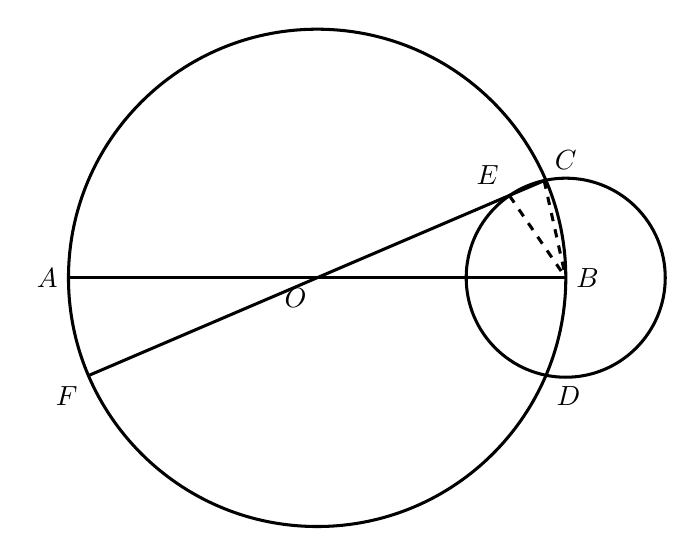
\begin{tikzpicture}[line width=1.1pt, line join=round]
\coordinate (A) at (-3.539,0.013);
\coordinate (B) at (2.777,0.013);
\coordinate (C) at (2.503,1.246);
\coordinate (F) at (-3.286,-1.231);
\coordinate (O) at (-0.380,0.011);



\coordinate (E) at (2.063,1.054);   
\coordinate (D) at (2.524,-1.228);  


\draw (O) circle[radius=3.158];     
\draw (B) circle[radius=1.264];     


\draw (A) -- (B);
\draw (F) -- (C);


\draw[dashed] (E) -- (B);
\draw[dashed] (C) -- (B);


\node[left] at (A) {\fontsize{10}{12}\selectfont$A$};
\node[right] at (B) {\fontsize{10}{12}\selectfont$B$};
\node[above right] at (C) {\fontsize{10}{12}\selectfont$C$};
\node[below right] at (D) {\fontsize{10}{12}\selectfont$D$};
\node[above left] at (E) {\fontsize{10}{12}\selectfont$E$};
\node[below left] at (F) {\fontsize{10}{12}\selectfont$F$};
\node[below left] at (O) {\fontsize{10}{12}\selectfont$O$};
\end{tikzpicture}
\end{document}